%%%%%%%%%%%%%%%%%%%%%%%%%%%%%%%%%%%%%%%%%%%%%%%%%%%%%%%%%%%%%%%%%%%%%%%%%%%%%%%%%%%%%%%%%%%%%
%%									Chapitre Approche de partitionnement et de distribution des graphes
%%%%%%%%%%%%%%%%%%%%%%%%%%%%%%%%%%%%%%%%%%%%%%%%%%%%%%%%%%%%%%%%%%%%%%%%%%%%%%%%%%%%%%%%%%%%%
\chapter{  Model Checking}
	\minitoc
	\newpage

%%%%%%%%%%%%%%%%%%%%%%%%%%%%%%%%%%%%%%%%%%%%%%%%%%%%%%%%%%%%%%%%%%%%%%%%%%%%%%%%%%%%%%%%%%%%%
\section{Introduction} 
De nos jours, la vie des êtres humains dépend largement des systèmes informatiques qui remplissent des fonctions de plus en plus critiques. Ceci à augmenter la difficulté d'assurer le bon fonctionnement de ces systèmes afin d'éviter des conséquences qui peuvent s'avérer fatales, coûteuses et dramatiques \citep{Huckle2015}, \citep{Kanaracus2012}. Dès lors, il faut fournir des techniques de vérification et de validation efficaces et performantes qui garantissent la sûreté de fonctionnement de ces systèmes critiques et qui prennent en charge leurs complexités croissantes \citep{Ferrari1978}.

Les méthodes formelles apportent une solution à ce problème, car elles permettent de définir des modèles mathématiques décrivant  rigoureusement le comportement des systèmes. Elles les décrivent principalement à l'aide de langages formels adaptés et définis avec précision au niveau de la syntaxe et de la sémantique. Une fois décrit, elles peuvent prouver la correction du modèle en utilisant des méthodes de vérification formelle. La vérification consiste alors à s'assurer que l'ensemble des fonctionnements du système développé satisfait tous les besoins \citep{ClarkeWing1996}, \citep{Dsilva2008}.
 
Le model checking est une forme de vérification formelle des systèmes \citep{Cheng2006}, \citep{Wang2004}. Son principe est de vérifier que le modèle représentant le système, respecte bien les propriétés que l'on attend de lui, d'où le terme model checking. Les systèmes sont spécifiés par des formalismes tels que les automates temporisés \citep{AlurDill1994}, et les propriétés sont exprimées par des assertions dans une logique, par exemple la logique temporelle \citep{BenAri1983}. Bien que cette technique soit restreinte à des systèmes ayant un nombre fini d'états, elle permet une détection rapide et économique des erreurs dans des systèmes complexes. Parmi les outils les plus connus, on peut citer UPPAAL, DiVine, CADP, Murphi, Roméo, SPIN \citep{Behrmann2004}, \citep{Barnat2010}, \citep{Garavel2013}, \citep{Dill1996}, \citep{Lime2009}, \citep{Holzmann2003}.

Les réseaux de Petri sont des outils à la fois graphiques et mathématiques permettant de modéliser le comportement dynamique des systèmes à  évènements discrets. Leur représentation graphique permet de visualiser d'une manière naturelle le parallélisme, la synchronisation, le partage de ressources, les choix (conflits), etc. Leur représentation mathématique permet d'analyser le modèle pour étudier ses propriétés    et de les comparer avec le comportement du système réel. L'une des approches de vérification d'un réseau Petri consiste à générer son graphe de marquage dont les sommets représentent les états dans lesquels le système peut se trouver, et dont les arcs représentent les transitions faisant passer le système d'un état à un autre. Après la génération, le graphe de marquage peut être vu comme un système de transitions étiquetées \citep{Arn92}. Le système de transitions étiquetées, ainsi généré, est utilisé pour la vérification des propriétés du système spécifié par le réseau (model checking, bissimilarité, test de conformité, etc. \citep{CES86}, \citep{FM}, \citep{CH93}). Cependant, le modèle des systèmes de transitions étiquetées fait abstraction quant à l'exécution parallèle des transitions.


Nous nous intéressons dans ce chapitre, au réseaux de Petri et au model checking distribuée. Nous présentons dans un premier lieu  les réseaux de Petri, puis les systèmes de transitions étiquetées et aussi la structure de Kripke. Enfin, on termine avec le model checking distribué.

\section{Réseaux de Petri}
Les Réseaux de Petri (abréviation  RdP) ont été introduits par le mathématicien Allemand Carl Adam Petri dans sa thèse \citep{Carl1962}, d'où leur appellation Réseaux de Petri (ou Petri Nets en anglais). Ces derniers méritent bien leur  appellation  car  la  thèse de C.A Petri a présenté un certain nombre d'idées fondamentales du modèle. Mais la théorie des RdP en sa totalité, telle que nous la connaissons actuellement est le résultat de fusionnement et de contribution directe ou indirecte des travaux de plusieurs  chercheurs de différentes universités et de différents laboratoires \citep{Robert2007}.

Les réseaux de Petri sont des outils à la fois graphiques et mathématiques permettant de modéliser le comportement dynamique des systèmes à  évènements discrets et d'évolutions simultanées. Leur représentation graphique permet de visualiser d'une manière naturelle le parallélisme, la synchronisation, le partage de ressources, les choix (conflits), etc. Leur représentation mathématique permet d'analyser le modèle pour étudier ses propriétés et de les comparer avec le comportement du système réel.

Cette section présente les notions fondamentales des réseaux de Petri.

\begin{definition}[Informelle]
Un réseau de Petri est un graphe biparti dont les sommets sont répartis selon deux types,  les places et les transitions. Ce graphe est constitué de telle sorte que les arcs du graphe ne peuvent relier que des places aux transitions ou des transitions aux places. Les places sont représentées par des cercles, alors que les transitions sont représentées par des traits ou des rectangles (Figure \ref{rdp}). Les places servent  à représenter les états du  système modélisé, tandis que les  transitions  représentent les changements d'état ou les événements \citep{SaidounicoursRdp2017}.

\begin{center}
	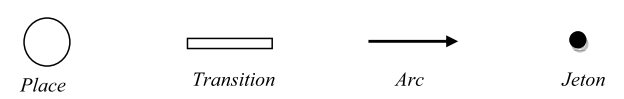
\includegraphics[scale=0.5]{img/rdp.PNG}
	\captionof{figure}{Représentation graphique des éléments d'un RdP} \label{rdp}
\end{center}


 Chaque place peut contenir un nombre entier de jetons. Les jetons modélisent souvent l'état d'une ressource (nombre d'instances, occupée ou non, ...). Un jeton est représenté par un petit cercle noir. Pour des commodités de présentation on met à l'intérieur d'une place le nombre de jetons présents (Figure \ref{place}). 
 
 \begin{center}
	
\includegraphics[scale=0.5]{img/place.PNG}
	\captionof{figure}{ Marquage d’une place } \label{place}
 \end{center}

 À  chaque arc est associé un nombre entier strictement positif appelé poids de l'arc. Lorsque le poids n'est pas signalé, il est égal à $"1"$  par défaut. Le RdP dont tous ses arcs sont de poids "1" est appelé RdP ordinaire (Figure \ref{rdpo}). Dans le cas o\`{u} les arcs peuvent avoir des poids supérieurs à $"1"$, il s'agit de RdP généralité (Figure \ref{rdpg}).
 
 \begin{center}
	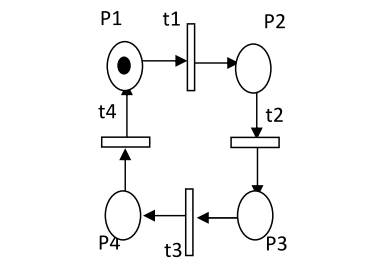
\includegraphics[scale=0.5]{img/rdp1.PNG}
	\captionof{figure}{RdP ordinaire} \label{rdpo}
 \end{center}
 
 \begin{center}
	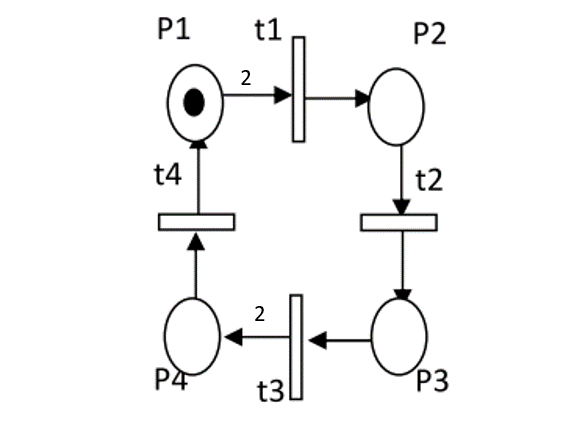
\includegraphics[scale=0.5]{img/rdpg.PNG}
	\captionof{figure}{RdP généralité} \label{rdpg}
 \end{center}
\end{definition}

\begin{definition}[Formelle]\citep{Murata1989}\\
Formellement un RDP est un quintuplet, $R= (P, T, Pre,Post , M_0 )$ tel que:
\begin{itemize}
	\item P : L'ensemble des places;
	\item T : L'ensemble des transitions;
	\item Pre : $(P  \times T)\rightarrow IN$, est l'application d'incidence avant, correspondant aux arcs directs reliant les
places aux transitions;
	\item Post : $(T  \times P)\rightarrow IN$,est l'application d'incidence arrière, correspondant aux arcs directs reliant
les transitions aux places;
	\item La matrice incidence du réseau est $C=Post-Pre$;
	\item $M_0$ : Le marquage initial (état initial). 
\end{itemize} 
\paragraph{Notation}
\begin{itemize}
	\item °t : L'ensemble des places d'entrée de la transition t;
	\item t° : L'ensemble des places de sortie  de la transition t;
	\item °p : L'ensemble des transitions  d'entrée de la place p; 
	\item P° : L'ensemble de transitions de sortie de la place p;  
\end{itemize}
Le RdP de la Figure \ref{rdp1} décrit le cycle des quatre saisons. Les places représentent les saisons,   $p_1$; le printemps, $p_2$; l'été,   $p_3$: l'automne et $p_4$: l'hiver. Les transitions représentent les changements de saisons, $t_1$; le début d'été, $t_2$; le début d'automne, $t_3$: le début d'hiver et $t_4$: le début du printemps. Le jeton dans la place $p_1$ indique que la saison à l'instant initial est le printemps. Ce scénario est modélisé comme suit:\\ 
$P= \{p 1 , p 2 , p 3 , p 4 \}$,\\ 
$T= \{t 1 , t 2 , t 3 , t 4 \}$, \\  
$Pre(p_1 ,t_1 )=1,\;\; 
Post(t_1 ,p_2 )=1,\;\; 
Pre(p_2 ,t_2 )=1,\;\; 
Post(t_2 ,p_3 )=1,\;\; 
Pre(p_3 ,t_3 )=1,\\ 
Post(t_3 ,p_4 )=1,\;\; 
Pre(p_4 ,t_4 )=1,\;\; 
Post(t_4 ,p_1 )=1$ ,  \\
$^{\circ}t_1=\{p_1 \},\;\; 
t_1^{\circ} =\{p_2 \},\;\; 
^{\circ}t_2=\{p_2 \},\;\; 
t_2^{\circ} =\{p_3 \},\;\; 
^{\circ}t_3=\{p_3 \},\;\; 
t_3^{\circ}=\{p_4 \},\;\; 
^{\circ}t_4=\{p_4 \},\;\; 
t_4^{\circ} =\{p_1 \}$,\\
$^{\circ}p_1= \{t_4 \},\;\; 
p_1^{\circ} = \{t_1 \},\;\; 
^{\circ}p_2= \{t_1 \},\;\; 
p_2^{\circ} =\{t_2 \},\;\; 
^{\circ}p_3= \{t_2 \},\;\; 
p_3^{\circ} = \{t_3 \},\;\; 
^{\circ}p_4= \{t_3 \},\;\; 
p_4^{\circ} = \{t_4 \}$.
 \begin{center}
	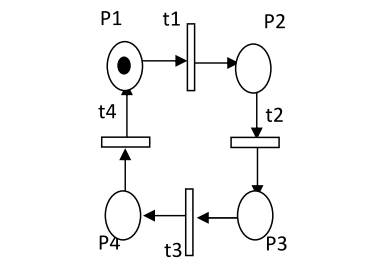
\includegraphics[scale=0.5]{img/rdp1.PNG}
	\captionof{figure}{Réseaux de Petri de quatre saisons} \label{rdp1}
 \end{center}
\end{definition}

\begin{definition}[Sensibilisation d'une transition]
Une transition $t$ est dite sensibilisée (validée, franchissable ou tirable) si chacune des places d'entrée $p$ contient un nombre de jetons supérieur ou égal au poids de l'arc reliant $p$ à $t$ \citep{SaidounicoursRdp2017}.  
$$ \forall p \in P, M(p) \geq  Pre (p, t) $$
\end{definition}

\begin{definition}[Franchissement d'une transition]
Le franchissement d'une transition $t$ sensibilisée retire de chacune de ses places d'entrée $p$ un nombre de jetons égal au poids de l'arc reliant $p$ à $t$ $(Pre (p, t))$ et dépose sur chacune de ses places de sortie p un nombre de jetons égal au poids de l'arc reliant $t$ à $p$ $(Post (p, t))$ \citep{SaidounicoursRdp2017}. Le franchissement d'une transition dans un marquage $M$ donne un nouveau marquage $M'$ défini par:
$$ \forall p \in P : M'(p)= M(p)+ C(p,t) $$

La Figure \ref{atom} illustre la réaction chimique $(2H_{2} + O_{2} \rightarrow 2H_{2}O)$ et le changement de marquage après le franchissement de la transition $t$. Avant le franchissement $M_ 0 =[2\; 2\; 0]$, après le franchissement $M_1 =[0\; 1\; 2]$. Les places sont ordonnées dans ce vecteur comme suit: $H_2 , O_2 , H_2 O$, le marquage de la place $H_2$ est noté par $M(H_2 )$. $M_0 (H_2 )$ est le marquage initial de la place $H_2$. Dans cet exemple $M_0 (H_2 ) =2$. 

\begin{center}
	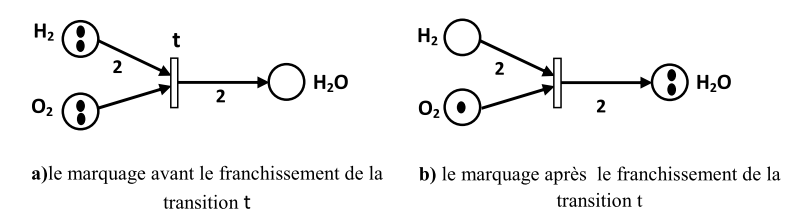
\includegraphics[scale=0.5]{img/H2O.PNG}
	\captionof{figure}{La composition d'eau $(2H_{2} + O_{2} \rightarrow 2H_{2}O)$ sous forme d'un RdP} \label{atom}
 \end{center}
\end{definition}\paragraph{Remarque }
 Lorsqu'une transition est validée, cela n'implique pas qu'elle sera immédiatement franchie; cela ne représente qu'une possibilité de franchissement, dans un  RdP, même si plusieurs transitions sont validées par un même marquage une et seulement une transition peut être franchie.
 
 
\begin{definition}[Graphe des Marquages]
Le graphe des marquages du réseau $G(R, M_0 )$ est défini par un graphe orienté dont les sommets sont étiquetés par les marquages des états accessibles $Acc(R, M_0 )$ et dont les arcs sont étiquetés par des transitions de $L(R, M_0 )$.
Un marquage $M_i$  est accessible (atteignable) à partir de $M_0$ , s'il existe une séquence $s$ de franchissement de transitions qui permet d'atteindre $M_i$  à partir de $M_0$. On note: $M_0  [s > M_i  $


La construction du graphe des marquages $G$ est faite comme suit \citep{SaidounicoursRdp2017}:
\begin{itemize}
	\item Pour chaque marquage $M$ obtenu à partir de $M_0$, trouver toutes les transitions franchissables $t_i$;
	\item Pour chaque transition $t_i$, trouver son marquage $M’$;
	\item Construire le nouveau nœud s'il est différent de ceux déjà obtenus, puis ajouter l'arc correspondant au marquage actuel vers le prochain;
	\item Continuer l'exploration tant que des marquages et des transitions n'ont pas été encore considérés.
\end{itemize}
La Figure \ref{gm1} illustre le graphe des marquages obtenue à partir du RdP de la Figure \ref{atom}.
\begin{center}
	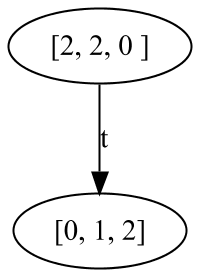
\includegraphics[scale=0.4]{img/gm1.png}
	\captionof{figure}{Graphe des marquages de $(2H_{2} + O_{2} \rightarrow 2H_{2}O)$} \label{gm1}
 \end{center}
\end{definition}

\begin{definition}[Système de transitions étiquetées]
Un système de transitions étiquetées appelé aussi $STE$ est un graphe orienté dont les sommets et les arcs de ce graphe orienté sont appelés respectivement états et transitions. Ces états et transitions sont associés avec une chaîne de caractères de manière à pouvoir les  distinguer entre eux.  Ces chaînes de caractères s'appellent \emph{noms} lorsqu'elles sont associées aux états, et étiquettes lorsqu'elles sont associées aux transitions .


Formellement un système de transitions étiquetées  est un quadruplet $\; STE = (S, Act, \delta, s_0)$ \citep{Saidouni2012}:
\begin{itemize}
	\item\textbf{S} est un ensemble (dénombrable) d'états;
	\item \textbf{Act}  est un ensemble (dénombrable) d'actions dites observables; 
 	\item  $\delta\subseteq \; S \times (Act \cup \{i\})$ : est l'ensemble des transitions, $i \notin Act$ est appelée action invisible (interne ou non-observable). Un élément $(x, a, y) \in \delta $ sera aussi noté par $x \stackrel{a}{\rightarrow}y$.
 	\item $s_0$ $\in\; S$ est l'état initial de $STE$. 
\end{itemize}

La Figure \ref{ste} illustre le STE du graphe de marquage de la Figure \ref{gm1}.
\begin{center}
	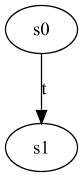
\includegraphics[scale=0.4]{img/ste.png}
	\captionof{figure}{STE de $(2H_{2} + O_{2} \rightarrow 2H_{2}O)$} \label{ste}
 \end{center}
\end{definition}

\begin{definition}[Structure de Kripke]
Une Structure de Kripke est un graphe orienté dont les nœuds représentent les états accessibles du système et dont les arcs représentent les transitions entre les états. Une fonction d'étiquetage fait correspondre à chaque état un ensemble de propositions logiques vraies dans cet état \citep{Kripke1963}.

Formellement une structure de Kripke est un 4-uplet ${\displaystyle M=(S,I,R,L)}$ \citep{Edmund1999}:
\begin{itemize}
	\item \textbf{S} est un ensemble fini d'états;
	\item \textbf{I} $\subseteq$ \textbf{S} est un ensemble d'états initiaux;
	\item \textbf{R} $\subseteq$ \textbf{S}$\times$\textbf{S}  est une relation de transition qui vérifie: pour tout ${\displaystyle s\in S}$, il existe ${\displaystyle s'\in S} $ tel que ${\displaystyle (s,s')\in R}$;
	
Soit ${\displaystyle AP}$ un ensemble de propositions atomiques, c'est-à-dire des expressions booléennes portant sur des variables, des constantes et des prédicats. On note ${\displaystyle 2^{AP}} $ l'ensemble des parties de ${\displaystyle AP}$.
	\item \textbf{L: S} $\rightarrow 2^{AP}$ est une fonction d'étiquetage(ou d'interprétation) définit pour chaque état ${\displaystyle s\in S}$ l'ensemble ${\displaystyle L(s)}$ de toutes les propositions atomiques qui sont valides dans cet état.
\end{itemize}

\paragraph{Remarque}
La condition associée à la relation de transition ${\displaystyle R}$ spécifie que chaque état doit avoir un successeur dans ${\displaystyle R}$, ce qui implique que l'on peut toujours construire un chemin infini dans la structure de Kripke. Cette propriété est importante lorsque l'on traite des systèmes réactifs\citep{Klaus2004}. Pour modéliser un interblocage dans une structure de Kripke, il suffit de faire boucler l'état d'interblocage sur lui-même.


Un chemin dans la structure ${\displaystyle M}$ est une suite ${\displaystyle c=s_{1},s_{2},s_{3},\ldots }$ d'états tels que ${\displaystyle (s_{i},s_{i+1})\in R}$ pour tout ${\displaystyle i}$. L'étiquette du chemin est la suite d'ensembles ${\displaystyle w=L(s_{1}),L(s_{2}),L(s_{3}),\ldots }$,$\ldots$ qui peut être vu comme un mot infini sur l'alphabet ${\displaystyle 2^{AP}}$.

\end{definition}

La Figure \ref{stkrdp} représente une structure de Kripke dont l'ensemble de propositions atomiques est ${\displaystyle AP=\{p,q\}}$. Ici ${\displaystyle p}$   et ${\displaystyle q}$  sont des propriétés booléennes quelconques. L'état \emph{$s_1$} contient les deux propositions, les états \emph{$s_2$} et \emph{$s_3$} respectivement ${\displaystyle q}$  et ${\displaystyle p}$. L'automate admet le chemin ${\displaystyle c=s_1,s_2,s_1,s_2,s_3,s_3,s_3,\ldots }$, et le mot ${\displaystyle w=\{p,q\},q,\{p,q\},q,p,p,p,\ldots }$ est la suite des étiquettes associées.

\begin{center}
	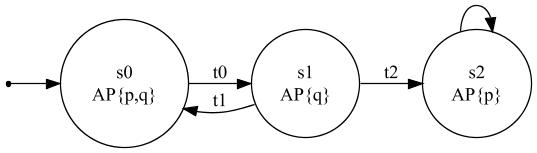
\includegraphics[scale=0.4]{img/stk.png}
	\captionof{figure}{Une structure de Kripke à trois états, avec deux propositions} \label{stkrdp}
 \end{center}
 
 
La distribution de l'espace d'états entraine la fragmentation de la structure de Kripke. Les structures partielles de Kripke modélisent des espaces d'états incomplets à parties inconnues (états border). L'évaluation des formules logiques temporelles sur les structures partielles de Kripke repose donc sur des interprétations à trois valeurs; la valeur de vérité supplémentaire \textbf{$\perp$ }  signifie « inconnu si la propriété est vraie ou fausse ».\\
Formellement une structure partielle de Kripke est un 4-uplet \\${\displaystyle F_M(T) = (S_T , I_T , R_T , L_T )}$ \citep{depriester2011bouneb}:
\begin{itemize}
	\item $T \subseteq S $;
	\item \textbf{$S_T$}  est une sous ensemble d'états fini de l'espace d'états S;
	\item \textbf{$R_T$} $\subseteq$ \textbf{$S_T$}$\times$\textbf{$S_T$}  est une relation de transition qui vérifie: pour tout ${\displaystyle s\in T}$, il existe ${\displaystyle s'\in S_T} $ tel que ${\displaystyle (s,s')\in R}$;
	\item $I_T$ est un ensemble fini d'états qui vérifie: pour tout $ s \in S_T $ tel que $ s \in I \}$;
	\item $ L_T$ : $S_T \times P \rightarrow \{ false, \perp , true \} $.
\end{itemize}

La Figure \ref{stkrdpd} représente des structures partielles de Kripke reparties sur trois machines, dont l'ensemble de propositions atomiques est ${\displaystyle AP=\{a,b,c\}}$. La répartition des états est faite comme suit:  
\begin{itemize}
 \item Sur la machine $M_1$ la structure partielle renferme deux états à parties complètes $s_0$ et $s_1$, et deux états à parties incomplètes $s_2$ et $s_4$;
 \item Sur la machine $M_2$ la structure partielle renferme un état à partie complète $s_4$, et un état à partie incomplète $s_5$;
 \item Sur la machine $M_3$ la structure partielle renferme deux  états à parties complètes $s_2$ et $s_5$, et deux états à parties incomplètes $s_1$ et $s_4$
 \end{itemize}

\begin{center}
	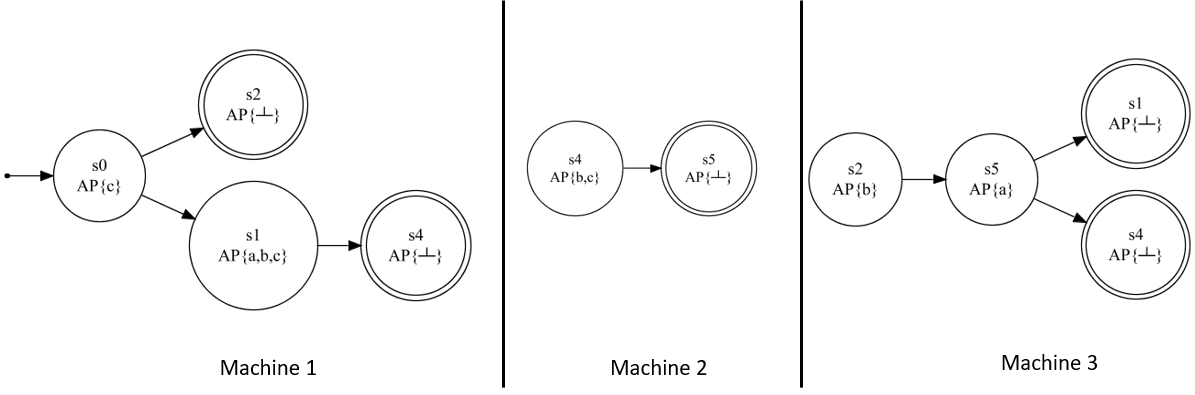
\includegraphics[scale=0.7]{img/stkd.png}
	\captionof{figure}{Structure de Kripke distribuée de cinq états, avec trois propositions} \label{stkrdpd}
 \end{center}
\section{Logique temporelle arborescente (CTL)}
Logique temporelle définie des opérateurs permettant de \s{lier} des variables propositionnelles \emph{p} aux instants \emph{t}. Par exemple, une assertion liée au comportement d'un programme telle que \s{après exécution d'une instruction i, le système se bloque}, les actions de cette assertion s'exécutent suivant un axe de temps : à l'instant \emph{t}, exécution de l'instruction \emph{i}, et à \emph{$t + 1$} blocage du système. La logique du temps arborescent permet de modéliser les expressions du passé et du futur \citep{Bakker1983}, \citep{Clarke1981}, \citep{Emerson1983}.\\

La logique du temps arborescent (CTL) « Computation Tree Logic (en aglais) » permet d'exprimer des propriétés portant sur les arbres d'exécution (issus de l'état initial) du programme. Elle modélise des expressions du passé et du futur à partir d'un état du système. Une expressions CTL exprime des propriétés relatives à l'arbre d'exécution grâce une syntaxe et une sémantique.

\subsection{Syntaxe de CTL}
Le langage des formules de CTL sont les formules d'état définies inductivement par:
\begin{itemize}
	\item  $ \forall p \in AP$, p est une formule d'état;
	\item  Si p, q sont des formules d'état, alors $p \vee q$ et $\neg p$ sont des formules d'état;
	\item Si p est une formule de chemin, alors \emph{$E_p$} et \emph{Ap} sont des formules de chemin;
	\item Si p et q sont des formules d'état, alors \emph{$X_p$} et \emph{pUq} sont des formules d'état.
\end{itemize}

\subsection{Sémantique de CTL}
La sémantique de CTL est interprétée dans une structure de Kripke. Les états sont décorés par les propositions atomiques ${\displaystyle p}$.\\
Soit $q_0$ un état de S. La sémantique de CTL est définie inductivement par:
\begin{itemize}
	\item  $p \in AP$, $q_0 \models p \Leftrightarrow p \in L(q_0 )$
	\item $q_0 \models p\vee q \Leftrightarrow q_0 \models p\; ou\; q_0 \models q$
	\item $q_0 \models \neg p \Leftrightarrow not(q_0 \models p)$
	\item  $q_0 \models Ep \Leftrightarrow  \exists \delta =q_0 …q_n$ telle que $\delta \models p$ (p formules de chemins)
	\item $q_0 \models Ap \Leftrightarrow \forall \delta =q_0 …q_n$ on a $\delta \models p$ (p formules de chemins)
	\item$ \delta \models Xp \Leftrightarrow \delta _1 \models p$ (p formules d'état)
	\item $ \delta \models pUq \Leftrightarrow \exists j \geq 0, \delta _j \models q\; et (\forall k <j, \delta _k \models p)$ (p et q formules d'état)
\end{itemize}
les opérateurs temporels sont définies par:
\begin{itemize}
	\item A (All), E (Exist): quantifications sur toutes les exécutions possibles à partir de l'état courant
	\item X (next), F (eventually), G (always),U précédent directement  A, E
	\item $\neg , \vee, \wedge$
\end{itemize}

Pour illustrer l'utilisation de la logique temporelle arborescence dans la formalisation des problèmes pratiques, nous donnons l'exemple du publiphone qui consiste à modéliser les actions qu'un utilisateur exécute pendant l'opération de tentative de téléphoner jusqu'à la fin de la communication. La procédure téléphonée est la suivante :
\begin{itemize}
	\item L'utilisateur doit décrocher le téléphone;
	\item Le système affiche insérer une carte;
	\item L'utilisateur insère une carte;
	\item Le système affiche le nombre d'unités restantes;
	\item L'utilisateur compose son numéro de téléphone avec la possibilité de le corriger pour obtenir le   bon numéro dans un délai de 2 secondes;
	\item L'utilisateur communique avec son correspondant, tant qu'il lui reste des unités. – Si la carte est épuisée, l'utilisateur a 10 secondes pour la changer;
	\item Lorsque la communication est terminée, l'utilisateur raccroche le téléphone;
	\item Le système affiche retirer la carte. – L'utilisateur retire sa carte;
\end{itemize}
Ensuite, formalisons les propositions atomiques :
\begin{itemize}
	\item u\_décrocher : l'utilisateur décroche le téléphone
	\item sys\_affiche(message) : le système affiche le message
	\item u\_insérer\_carte : l'utilisateur insère une carte
	\item u\_compser\_no : l'utilisateur compose le numéros
	\item u\_correction\_no : l'utilisateur corrige le numéros
	\item numéros\_correct : le numéros est correct
	\item u\_communiquer : l'utilisateur communique avec son correspondant
	\item u\_changer\_carte\_vide : l'utilisateur change sa carte qui est épuisée
	\item u\_raccrocher : l'utilisateur raccroche le téléphone
	\item u\_retirer\_carte : l'utilisateur retire sa carte
	\item ctl\_téléphoner : établit la clause de l'activité téléphoner
\end{itemize}

Enfin, on obtient la formalisation en CTL:\\

$u\_decrocher \; \wedge\; u\_inserer\_carte \wedge 	\\
AX [(u\_composer\_no\; \wedge\; EF (u\_reprise\_sur\_erreur)) \wedge \\
AX ((u\_communiquer \;\wedge\; EF (changer\_carte\_vide)) U \\
(u\_raccrocher \;\wedge \; u\_retirer\_carte))] \Rightarrow \; ctl\_telephoner$
\section{Model checking}
Le model checking peut-être ramené à la vérification d'une propriété \emph{P} sur un système $\phi : \phi \models P$. Plusieurs types de propriétés peuvent être vérifiés tels que les propriétés de sûreté ou de vivacité. Toutefois, vérifier des propriétés de sûreté est très souvent suffisant : On peut détecter des interblocages, vérifier des bornes ou encore qu'une section critique est bien respectée par les processus y accédant. 


Vérifier une propriété de sûreté revient à parcourir les états que peut atteindre un système, et pour chaque état rencontré, vérifier si la propriété est respectée. Il s'agit donc d'un parcours de graphe (en largeur ou en profondeur).

Ainsi, la génération distribuée de l'espace d'états permet de répartir l'ensemble des états entre les machines du réseaux, ce qui permet de pallier au problème de l'explosion combinatoire de l'espace d'états. Le but de cette génération distribuée est la vérification de systèmes de tailles importantes. De ce fait, les algorithmes de vérification feront aussi l'objet de distribution. 

L'algorithme de model checking distribué qui a été développé dans \citep{depriester2011bouneb}, elle représente un version simplifiée de l'algorithme de model checking distribué. Toutes les machines contribuent pour la vérification des propriétés exprimées en CTL. Chaque machine vérifiée la propriété sur la structure de Kripke partiale, la vérification au niveau des états à parties inconnues est traité indécidable. Ainsi, les machines coopèrent afin de vérifier la formule CTL. 

Dans cette section, nous présentons L'algorithme de model checking distribué qui a été proposer dans \citep{depriester2011bouneb}.

\subsection{Model checking CTL  sur les fargments}
Soit $M = (S, L, R, I)$ un fragment de structure de Kripke et une formule de CTL, l'algorithme récursif suivant calcule l'ensemble des états $H(f) \subseteq S$ qui satisfont f ou elle peut satisfaire f et qui exclut tous les états qui ne satisfont pas f. 
 \begin{flalign}
    \label{eqn1}
	&  T(p)= \left\{ x \in S\mid(x,p)=true\right\}&  \\
	\label{eqn2}
	&  U(p) = \left\{ x \in S\mid(x,p)=\bot\right\} \\
	&  F(p) = \left\{ x \in S\mid(x,p)=false\right\} \label{eqn3}
\\
	&  pour \; x \;\in T,inT(x) = (1,x) \label{eqn4}
\\
&	T^+(p)=\left\{ inT(x)\mid \forall x \in T\right\}\label{eqn5}
\\
&	pour \; x\; \in U,inU(x)=(-1,x) \label{eqn6}
\\
&	 U^+(p)=\left\{ inU(x)\mid \forall x \in U\right\}\label{eqn7}
\\
&	pour \;x \; \in F,inF(x)=(0,x) \label{eqn8}
\\
&	F^+(p)=\left\{ inF(x)\mid \forall x \in F\right\}\label{eqn9}
\\
&	S^+(p)=T^+(p)\cup U^+(p)\cup F^+(p)\label{eqn10}
\\
&	H(p)=T^+(p)\cup U^+(p); \;p\; une\; proposition\; atomique\label{eqn11}
\\
&	H(\ne f)=\left\{ inT(x)\mid x\in (S-map(snd,H(f)))\cup U^+(f)\right\}\label{eqn12}
\\
&	H(f\wedge g)=H(f)\sqcup H(g) \label{eqn13}
\\
&	H(f\vee g)=H(f)\sqcap H(g)\label{eqn14}
\\
&	H(AXf)=\left(\left\{inT(snd(e))\: \mid \forall\; e \; \in S^+(f).succ(e) \;\subseteq\; T^+(f)\; \subseteq\; H(f) \right\} \;\cup\atop \left\{inU(snd(e))\: \mid \forall \;e\; \in S^+(f).succ(e)\; \subseteq\; (T^+ (f)\;\cup\atop U^+(f))\; and\; \exists \;e' \;\in \;succ(e) \;telque\: e'^+(f)\right\}\right)\atop \sqcup\left\{inU(x) \mid x \in border(M) \right\}\label{eqn15}
\\
&	H(EXf)=\left(\left\{inT(snd(e))\: \mid \forall\; e' \; \in S^+(f).succ(e) \;\subseteq\; T^+(f) \right\} \;\cup\atop \left\{inU(snd(e))\: \mid \forall \;e'\; \in S^+(f).succ(e)\; \subseteq\; U^+(f)\subseteq\; H(f)\right\}\right) \sqcup\atop\left\{inU(x) \mid x \in border(M) \right\}\label{eqn16}
\\
&	H(AGf)=vZ.((H(f)\sqcap AXZ) \label{eqn17}
\\
&	H(AFf)=\mu Z.(H(f)\sqcup AXZ)\label{eqn18}
\\
&	H(A(f\cup g)=\mu Z.(H(g)\sqcup H(f))\label{eqn19}
\end{flalign}

Après l'application de l'algorithme récursif ci-dessus, nous avons $\forall s \notin H(f) \Rightarrow L(s, f) =false$. Les autres opérateurs, comme par exemple $EG$ peuvent être déduites de l'ensemble des opérateurs cités ci-dessus, par exemple $H(EGf) = H( \neg (AF \neg f))$.

\subsection{Model checking CTL  distribué}
l'algorithme model checking distribué considère l'ensemble de la formule \\$\phi \in \{ f EGf, AGf, AFf, EFf, A(fUg), E(fUg) \}$ peut-être vérifiée dans les états border et aussi la vérité sur les états border est le paramètre passé au transformateur de
prédicat  comme suit :

 \begin{flalign}
 & Y =  \{ s \in  border(M) \mid  L(s, \phi) = True ou L(s, \phi) = \bot \} \phi \; est \; une \; formule  &\\
 & AFp = \lambda Y. \mu Z.(p \vee Y \vee  AXZ)\\
 & AGp = \lambda Y.\mu Z.(p \vee Y \wedge  AXZ)  \\
 & EGp = \lambda Y.\mu Z.(p \vee Y \wedge EXZ) \\
 & A(p \cup q) = \lambda Y.\mu Z.(q \vee Y \vee(p \wedge AXZ)) \\
 & E(p \cup q) = \lambda Y.\mu Z.(q \vee Y \vee (p \wedge EXZ)) \\
\\
\end{flalign}

\emph{Y} représente l'absence d'information sur l'état border, grâce  à l'information obtenue au niveau des états border,  la validitée de la formule peut être conclus sur toute la structure de Kripke.
\section{Conclusion}{
Dans ce chapitre, nous avons présenté les réseaux de Petri ainsi que les systèmes de transitions étiquetées et aussi la structure de Kripke. Ensuite nous avons présenté  la logique temporelle arborescente et le model cheching distribué qui exploite l'information au niveau des états du graph ainsi qu'il permet la vérification malgré l'insuffisance d'information résultante de la distribution de l'espace d'états sur plusieurs nœuds.